%!TEX root = project.tex

\chapter*{Preface}
This report is the documentation of the project work as part of the Bachelors (Honours) dissertation in Computing and Software Development - 2016 and marks the end of the four-year long Bachelors (Honours) Degree at Galway-Mayo Institute of Technology (GMIT). This is a 15 – credit module.

\paragraph{}
I would like to thank my supervisors, Mr Damien Costello, Dr John Healy, Dr Ian McLoughlin, for guidance and the feedback I’ve received throughout my work. 
I would also like to thank my family for their continuous support and encouragement throughout my years at the Galway-Mayo Institute of Technology.


\chapter{Introduction}
Over the past few years, mobile applications technology has developed rapidly and we have seen the tremendous improvements in mobile devices in terms of performance, additional hardware and software. 
Mobile applications technology has strong impacts in many areas of life such that nowadays, people rely on mobile apps for everyday life. This allows information to be available anywhere, anytime and accessible from all the devices.  The world has gone mobile so much that every person has access to a mobile device that they use not only to communicate with other people but also to access their favourite websites and content whenever they want, regardless of their physical location or computer access. Recent development in web and mobile technologies has influenced the developers to provide tourism based mobile application services. This emergent development of web tourism services has turned a significant number of travellers around the world to use mobile apps for planning and experiencing their travels, as an alternative tourist guide.
Tourism has become one of the biggest sectors in the world and as well attractive sector for mobile devices with which tourist spend considerable time planning their activities, both before and during their visits.

According to \cite{Tourism}, recent statistics shows that the tourism industry has contributed around 7 trillion US dollars tom the global economy annually, nearing eight trillion in 2015. The number is growing rapidly since the technology got advanced. Travel app guides have made an important contribution to this since tourists started using more of them to enhance their travel experience.
In this project I propose a tourist guide mobile application that provides tourist guidance services through mobile devices. 
Putting into consideration that Malawi is a small country, very quiet and peaceful amongst the countries in Africa, hence called “The Warm Heart of Africa”, has a lot to offer to tourists in terms of nature and its geographical position. According to recent developments in terms of insecurities that face tourists as a result of terror activities as they travel to some parts of Africa and elsewhere around the world, I thought to myself that this would be an opportunity for the government of Malawi to promote tourism to the best of its ability by making use of the available technological resources such as mobile tour guide apps.
In summer 2015, I visited, Malawi on a holiday trip where I had time to visit some places of interest around the country. I decided to share my ideas to interested parties working for the Ministry of Tourism. I introduced the idea of developing a mobile app that can be used to promote Malawi tourism. 
Malawi being one of the under- developed third worlds countries, is facing challenges in Information and Communication Technology (ICT) development due to poverty and skills shortage in this field.
As a result of this, they are unable to fund such a project and therefore, I decided that I could help build a tourism app (free of charge) as my college final year project, of which they agreed. 

\section{Purpose}

The app will be used by tourists to find hotels, fun spots to hang out at and look for upcoming events.  They may also find this app a useful tool for checking weather forecast and to plan events accordingly. Tourists will be able to find information and easily locate points of interest such as hotels, restaurants and wildlife reserves in order to let them schedule their time more efficiently and increase the probability that they will visit places that they'll actually enjoy while in Malawi. The app will allow the users to add their personalized contents such diary notes.	

\section{Goals and Objectives}
This application will provide a better user experience by taking advantage of newest technologies in order to promote Lake Malawi, mountains, wildlife reserves, cities, hotels, museums and the cultural heritage.

The app is developed to target two major mobile platforms such as Android OS and iOS. The main goal of this project is to have fully functional tourist app that can be used anywhere, anytime.  This application is intended to be a cross-platform mobile application that can run on multiple platforms. The data that is used by this application is retrieved from the backend (Database) service the first time the user uses the application. The data will be stored in the user’s mobile’s device (local storage) and made available at anytime for future use. In addition, the application will be capable of both off-line and on-line usage. On-line mode will allow the user to take advantage of Google interactive maps indicating certain locations. At the moment, this functionality is not available in off-line mode. The user still can use the application as data is already stored in the mobile’s cache memory (local database). All the functionalities described briefly above have implemented by using web programming and mark-up languages such as AngularJS, JavaScript, HTML5, CSS. Ionic framework has been used to develop the front-end of the mobile application. All these technologies are to be discussed later in the sections.

\section{Scope}
The mobile app development project has two main domains: Mobile application and Web application. The mobile version shall be used as front –end (ionic cross platform app) for the users to interact with. All of the data displayed on this version, will be served by the database. The web version will function as a front-end that will be used by Administrators to interact with the database that is being used to provide store, update or delete data consumed by the mobile application. 

\section{Project Brief}
Below is a brief explanation of the chapters that I will be highlight more about this project:

\subsection{Methodology}
This section describes the way I went about doing this project. This underpins my chosen research methods, product testing and also the interaction with the clients. 

\subsection{Technology Review}
This section is a brief description of technologies that I used during the entire development process. Also outlines the reason why I used such technologies and the as well providing references.

\subsection{System Design}
An overview of different components of the system, the architecture, including screenshots and diagrams, will be covered in this section.

\subsection{System Evaluation}
This section will describe ways in which I believe that the system is robust through testing techniques that were used to test the system. This will put into consideration space and time complexity for the system. It will also highlight any of the limitations or opportunities in the technologies used. 


\chapter{Methodology}
This section will describe the way I went about this project. I will shade light to research activities that I carried out in order to come up with a software development methodologies that perfectly suits the purpose of this project. I will also detail algorithms, languages, platforms and technology used and the procedures that I followed during testing and validation of the entire system.
To access the project application, please follow the links provided below:

\paragraph{}
\section{Research Activities}
Having considered all the necessary information from the client (user story), I conducted research on the latest technology that can be used to develop a robust application according to the user requirements. This was done through literature review on based on different conference papers, online journals website contents. 
According to \cite{Dawidowicz}, literature review method is an examination of information on specific subject. It is reviewing what is known and not what is assumed. It aims to create the final, precise representation of the knowledge and research-based theory available topic. When I learned that this project will involve working with databases, I had keen interest to figure out which database type best suites the purpose of this mobile app project. As part of my research module, I conducted a literature review \cite{NoSQL} from different literature review papers, publications, journals and citations that focused on the latest database technologies. In that paper, I examined the new generation of Not only Structured Query Language (NoSQL) databases that have arisen in order to cope with huge volumes of user data, products and objects that need to be stored and retrieved at the same time and at relatively high speeds. I discovered that these databases are thought to be flexible enough to cope with big data as they are schema-less, as compared to traditional relational databases. The types of NoSQL databases vary according to performance. I was able to evaluate some of the most popular NoSQL databases such as: MongoDB (Document Store databases), Cassandra, CouchDB (Document Store databases), PouchDB and HBase. I compared them in terms of performance based on workloads and time required to perform search, update, delete and insertion operations. 

\paragraph{}
I also conducted a research on AngularFire. AngularFire is the officially supported AngularJS binding for Firebase.  Firebase is a backend service that provides data storage, authentication, and static website hosting for your Angular app. The combination of Angular and Firebase provides a three-way data binding between your HTML, your JavaScript, and the Firebase database \cite{Firebase}. I decided to implement this technology into this project to act as a back-end service.

\section{Agile Development}
Throughout this project, I have used agile development methodology. I have learned that agile development methodology perfectly fits the purpose for this mobile app development.

\begin{center}    
	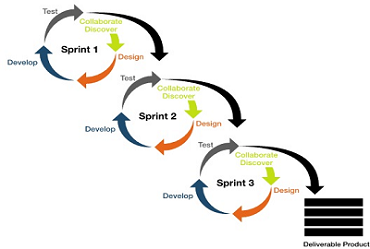
\includegraphics{img/agile.png}
\end{center}
\begin{center}
	Figure 1: Agile Methodology
\end{center}

\paragraph{}
Agile development, with its multiple cycles of testing and quality assurance, enables app developers to build in more quality. Reliability of agile comes as a result of repeated cycles of testing with each sprint. I have constant meetings with the client using Skype video call where I have to give updates on to the progress of the project. After thorough analysis of what I have done, they will give feedback which I use to further develop the app. All changes made to the app, are tested and then sent to the client as (discovermalawi.apk) file for verification.  In the case of web application, at the end of each development phase, the website is tested and then clients are able to verify if the websites functions as required. Any feedback is from them is taken on board to further develop the website. 
The advantage of Agile is that I have constant alliance with the client. This simply means that the client has the opportunity to request modifications to the product even at later stages of development.

\chapter{Technology Review}
Several technologies were used throughout the development of this project. This section briefly describes all of them and also emphasizes the reasons I chose to use them. 

\section{NodeJS}
Node.js is a JavaScript runtime built on Chrome's V8 JavaScript engine. Node.js uses an event-driven, non-blocking I/O model that makes it lightweight and efficient \cite{NodeJS}.
Node.js has the following the attributes:

\paragraph{Asynchronous and Event Driven}
\paragraph{}
All APIs of Node.js library are
asynchronous, that is, non-blocking. It essentially means a Node.js based
server never waits for an API to return data. The server moves to the next
API after calling it and a notification mechanism of Events of Node.js helps
the server to get a response from the previous API call.

\paragraph{Very Fast}
\paragraph{}
Being built on Google Chrome's V8 JavaScript Engine, Node.js
library is very fast in code execution.

\paragraph{Single Threaded but Highly Scalable}
\paragraph{}
Node.js uses a single threaded model with event looping. Event mechanism helps the server to respond in a non-blocking way and makes the server highly scalable as opposed to traditional servers which create limited threads to handle
requests. Node.js uses a single threaded program and the same program can provide service to a much larger number of requests than traditional servers like Apache HTTP Server \cite{NodeJS}.
\paragraph{No buffering}
\paragraph{}
Node.js applications never buffer any data. These applications simply output the data in chunks.


\section{AngularJS}
AngularJS was used to develop the application. AngularJS is a structural framework for dynamic web apps. It lets you use HTML as a template language and lets you extend HTML's syntax to express your application's components clearly and succinctly. Angular's data binding and dependency injection eliminate much of the code you would otherwise have to write. And it all happens within the browser, making it an ideal partner with any server technology.
AngularJS provides the web application with Model-ViewController
(MVC) capability. In contrast to the traditional
MVC architecture like SpringMVC, where the website is
rendered from the server side, with Angular the view is
generated in the browser using its Model which holds all the
required data. The controller takes care of the interactions
between the HTML page and Model. The upside here is, there
is no server side calls involved in these operations and
everything is done on the client side with cached data.
AngularJS abstracts the server calls to a separate layer to avoid code redundancy across multiple views for a gateway built
with pure HTML5, JavaScript and REST services. This enables
easier gateway maintenance while letting the developers focus
on additional features. It encourages developers to use
declarative programming for building the UIs and imperative
programming for business logic. Gateways are dynamic and rely on a rich supply of real-time data. Angular's feature to
manipulate the DOM automatically, takes the burden off the
developers when data changes periodically. It makes the view
lightweight, by decoupling the view rendering from the server
side \cite{AngularJS}. 


\section{Twitter Bootstrap}
Twitter Bootstrap is a powerful framework that provides a
set of CSS classes and JavaScript functions to ease the process
of front-end development. Its responsive design features enable
support for both mobile and desktop displays as shown in "Fig
1". The websites developed are cross-browser and device
compliant: the same site works well on both desktop and
mobile displays, which is increasingly important as mobile
usage overtakes traditional web access. Developer does not
have to work with CSS to make the website look attractive or
support responsive design principles unless necessary \cite{AngularJS}. 


\section{AngularFire}
AngularFire is the officially supported AngularJS binding for Firebase. The combination of Angular and Firebase provides a three-way data binding between your HTML, your JavaScript, and the Firebase database \cite{Firebase}.

\section{Firebase}
Firebase gained traction among developers who wanted to build applications quickly with immediate feedback they write code in one window and it renders in another. Firebase handles that automatically for you. Our servers manage millions of concurrent connections and billions of operations per month.
Firebase is the database that I have used for this project. Firebase is a real-time cloud data service and provides an API that stores and syncs data across multiple clients/ devices and it serves millions of users in no time. Firebase database is stored as JSON and synchronized in realtime to every connected client. When you build cross-platform apps with our Android, iOS, andJavaScript SDKs, all of your clients share one Firebase database and automatically receive updates with the newest data.
Different features and functionalities for Firebase are described in detail throughout this section \cite{Firebase}.

\subsection{Firebase Real-time Database}
Firebase's primary product is a realtime database which provides an API that allows developers to store and sync data across multiple clients. Firebase isn’t just any ordinary database. As a real-time, scalable backend, it provide the tools that developers need to quickly build rich, collaborative applications that can serve millions of users. In this architecture, apps only consists of static content and assets, and all the dynamic content and user data is stored and retrieved from Firebase. With fully Firebase-powered apps, user authentication can be handled by a simple login service which supports Facebook, Twitter, Github and Google; in addition to a regular email/password login scheme. Simple Login eliminates the need for you to write your own server-side authentication code. Firebase can sync data in milliseconds. All data is transferred over a secure SSL connection with a 2048-bit certificate. Firebase apps remain responsive regardless of network latency or Internet connectivity. All writes to a Firebase database will trigger local events immediately, before any data has been written to the server. Once connectivity is re-established, the client will receive any changes it missed, synchronizing it with the current server state. Most applications need to know the identity of a user. Knowing a user's identity allows an app to provide a customized experience and grant them permissions to access their data. The process of proving a user's identity is called authentication. Firebase provides a full set of authentication options out-of-the-box.
When a user authenticates to a Firebase app, firebase manages their session, ensuring that the user is remembered across browser or application restarts.
Also firebase apps have built-in support for logging in with email and password, social login providers such as Facebook, Google, Twitter, and GitHub, and single-session anonymous login. Apps that use Firebase's built-in auth services can handle user login entirely with client-side code, saving developer's time and the headache of operating their own backend.
Developers using the realtime database can secure their data by using the company's server-side-enforced security rules.     
\cite{FirebaseRealtime}. 

\section{Ionic Framework }
Ionic framework has been used to develop a frontend for the system. Ionic is a powerful HTML5 SDK that helps developers build native-feeling mobile apps using web technologies like HTML, CSS, and Javascript. Ionic is both a CSS framework and a Javascript UI library. It is focused mainly on the look and feel, and UI interaction of your app. Ionic currently requires AngularJS in order to work at its full potential. The CSS can stand on its own, but it is also built to be enhanced by the developer \cite{IonicFramework}. 


\chapter{System Design}
This section gives an overview of different components of the system architecture, and how they are all tied together. The goal of this section is to provide internal logic of each of the modules identified during system design. The diagram below shows how different modules have been put together.

\begin{center}    
	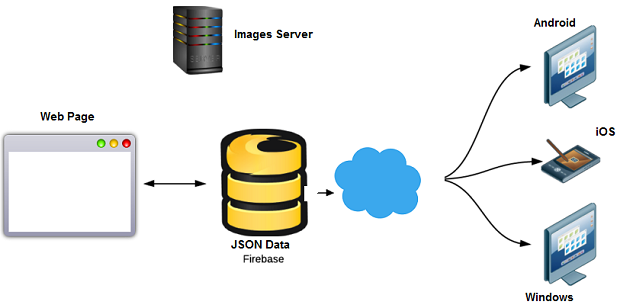
\includegraphics{img/diagram.png}
\end{center}
\begin{center}
	Figure 2: System Design
\end{center}
\paragraph{}
The Use Case diagram below indicates how the users and other software devices interact with the system.
\paragraph{}
\paragraph{}
\begin{center}    
	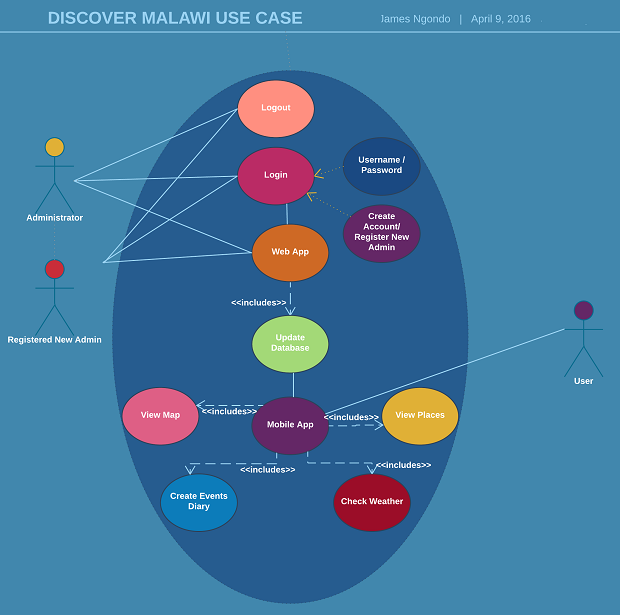
\includegraphics{img/UseCases.png}
\end{center}
\begin{center}
	Figure 3: System Use Case Diagram
\end{center}

\paragraph{}
The overall tourism application consists of broadly two units – the system backend and the ionic app (front end).

\section{System Backend}
The backend manages all the data that is being consumed by the frontend (Ionic App).The backend consists of three major components: Firebase database, administrator web application. The backend also uses Img Safe, an online free image storage server.

\subsection{Database}
Firebase is the database that I have used for this project. Firebase is a real-time cloud data service and provides an API that stores and syncs data across multiple clients/ devices and it serves millions of users in no time. Firebase database is stored as JSON and synchronized in realtime to every connected client. When you build cross-platform apps with Android, iOS, and JavaScript SDKs, all of the clients share one Firebase database and automatically receive updates with the newest data.
The following code snippet is used to pull data from firebase and display in the ionic app:

\begin{minted}{javascript}
  var app = angular.module('starter', ['ionic', 'ngCordova', 'firebase',
  'ngResource','ngStorage']);
  app.config(function($ionicConfigProvider){
	  $ionicConfigProvider.tabs.position('buttom');
  })
  var ref = new Firebase("https://discovermalawi.firebaseio.com/");
  
  app.factory('NoteStore', function($firebaseArray, $firebaseObject){
	  getAllParks: function(){  //get all parks
		 return $firebaseArray(ref.child('park'));
	  },
	  getPark: function(parkId){  //get individual park
		  return $firebaseObject(ref.child('park').child(parkId));
	  },
	  getAllLakes: function(){ // get all lakes
	  lakes = $firebaseArray(ref.child('lake'));
		  return lakes;
	  },
	  getLake: function(lakeId){ //get individual lake activites
		  return $firebaseObject(ref.child('lake').child(lakeId));
	  }  
  });
\end{minted} 
Different features and functionalities for firebase are described in detail throughout this section.

\subsubsection{Firebase Login}
The Administrator can directly login into the database. Firebase provides proper authentication. The admin will have to create/ register an account using their details (signup with Google). Once registered, the admin will have to login using either Google or typing in their email and password order to have access to the database. Successful login will direct the user to the application’s dashboard where they can be able to create a new database application or manage the existing database. The figure below shows the login form.

\begin{center}    
	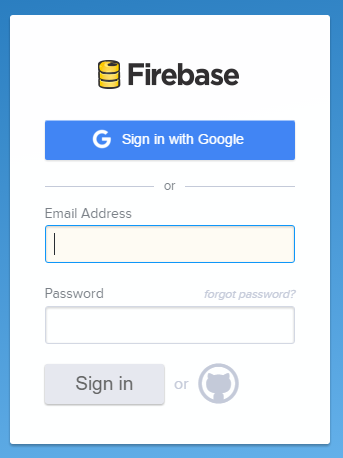
\includegraphics{img/firebaseLogin.png}
\end{center}
\begin{center}
	Figure 4: Firebase Login 
\end{center}

\subsubsection{Managing Existing Database}
In this case, “Discover Malawi” is being used as our database application. Upon clicking the “Manage App” button, the user is directed to the application’s main page where they can view all the contents of our database i.e. tables and data within the tables. The data in the database is stored as a JSON objects. The dashboard also has a functionality that allows the admin to export or import data in form of a JSON file. 

\begin{center}    
	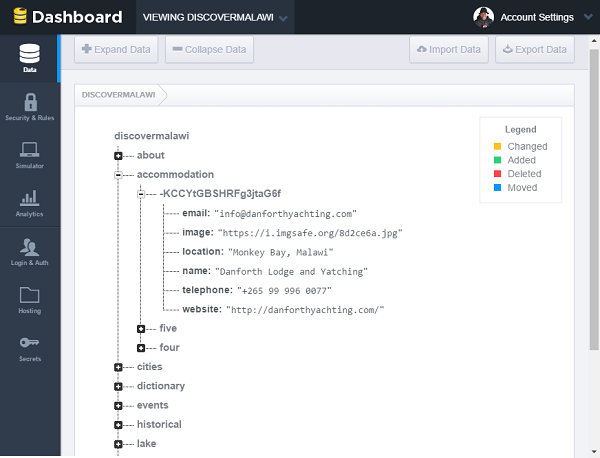
\includegraphics{img/dashboard.png}
\end{center}
\begin{center}
	Figure 5: Firebase - Admin Dashboard 
\end{center}

\paragraph{}
\subsubsection{Login And Authentication}
The dashboard also provides a functionality which allows admin (Database Administrator) to set login options and the length of sessions. In this case, the session has been set to 24 hours. This is the length of time the session will remain valid and this setting will affect all methods of authentication.
The admin has options to set domains (third-party) such as Facebook, Twitter, Github, Google for OAuth Redirects. This database has been set to accept only email and password to authenticate admin login. This is indicated in the figure below.

\begin{center}    
	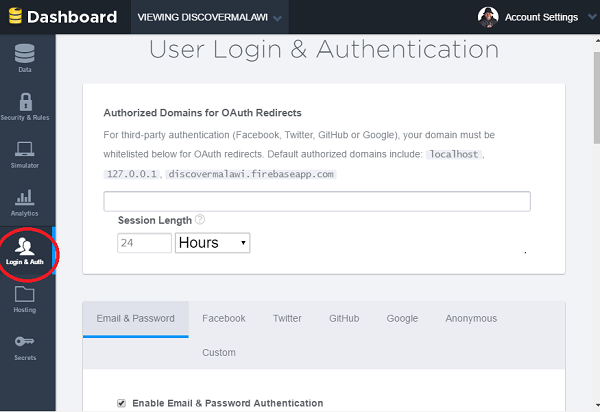
\includegraphics{img/userauth.png}
\end{center}
\begin{center}
	Figure 6: Firebase - User Authentication
\end{center}

\paragraph{}
\subsubsection{Password Reset}
The dashboard also provides the functionality that allows the admin to reset passwords for other registered administrators. In case of password reset, Firebase is designed to send a newly generated password direct to the user’s email. This enables password recovery in your app where users will be sent a new, temporary token that may be used to log in and update their credentials. The database is designed in such a way that the administrator can not see the user passwords as they are automatically encrypted. This is shown in the figure below. 
\begin{center}    
	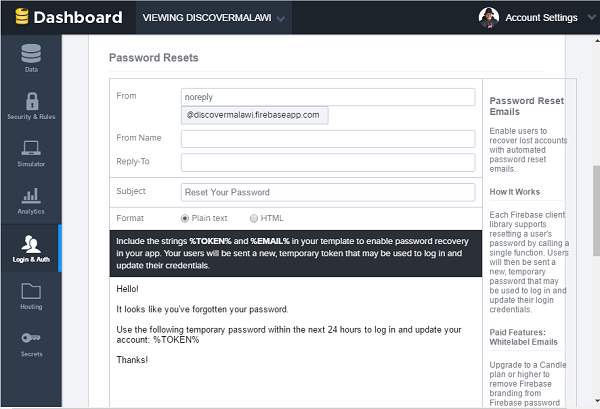
\includegraphics{img/passwd.png}
	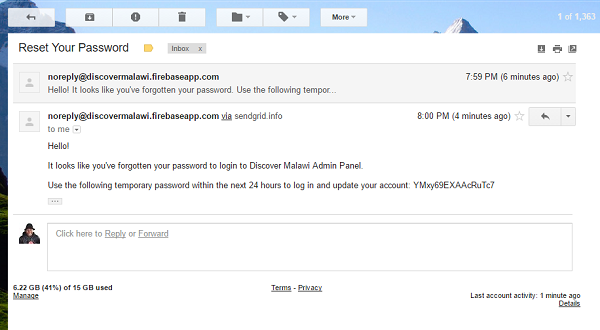
\includegraphics{img/passreset.png}
\end{center}
\begin{center}
	Figure 7: Firebase - Password Reset
\end{center}

\paragraph{}
\subsubsection{Add/ Delete User}
Using firebase, the admininstrator can also add, modify and delete other users using the dashboard. The dashboard also displays the list of all registered users, as shown in the figure below.
\begin{center}    
	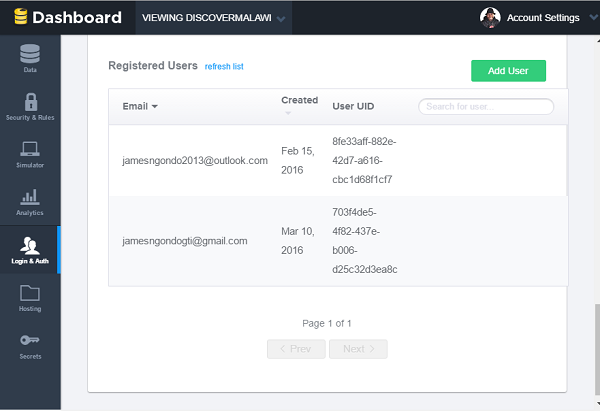
\includegraphics{img/delete_add.png}
\end{center}
\begin{center}
	Figure 8: Firebase - Add/ Delete Users
\end{center}

\paragraph{}
\subsection{Admin Web Application}
The web application is developed using AngularJS, HTML 5 and CSS. The web app is hosted live on Hosting24.com and can be accessed on\cite{hosting24}. The main purpose of the web app is to allow administrators interact with the database (Firebase). All CRUD (create, read, update and delete) operations to the database are performed using this web application and all the changes made to the database using the web app are updated on mobile apps in real-time. 

\subsubsection{Login Page}
Every single route in the web app is properly secured in such a way that the admin will have to login using a valid email and password in order to have access to data in the web app. Email and password entered is matched against the one that is registered in the Firebase. The code snippet below shows how the application connects to firebase for authentication and how the routes are protected:
\begin{minted}{javascript}
var myApp = angular.module('myApp', ['ngRoute', 'firebase'])
.constant('FIREBASE_URL', 'https://discovermalawi.firebaseio.com/');

myApp.run(['$rootScope', '$location',
function($rootScope, $location) {
	$rootScope.$on('$routeChangeError',
		function(event, next, previous, error) {
			if (error=='AUTH_REQUIRED') {
			$rootScope.message = 'Sorry, you must 
			log in to access that page';
			$location.path('/login');
		} // AUTH REQUIRED
	}); //event info
}]); //run
//=============Routes===========
 when('/register', {
	 templateUrl: 'views/register.html',
	 controller: 'RegistrationController',
	 resolve: {
		 currentAuth: function(Authentication) {
			return Authentication.requireAuth();
		 } //current Auth
	 } //resolve
 }).
  when('/about', {
	  templateUrl: 'views/about.html',
	  controller: 'AboutController',
	  resolve: {
		  currentAuth: function(Authentication) {
			  return Authentication.requireAuth();
		  } //current Auth
	  } //resolve
  }).
    
  otherwise({
  redirectTo: '/login'
  });
\end{minted}



All the input fields in this page are validated using AngularJS form validation as shown in figure below. 
For testing purposes, please use the following login details:
Username = g00304277@gmit.ie
Password = gmitgalway

\begin{center}    
	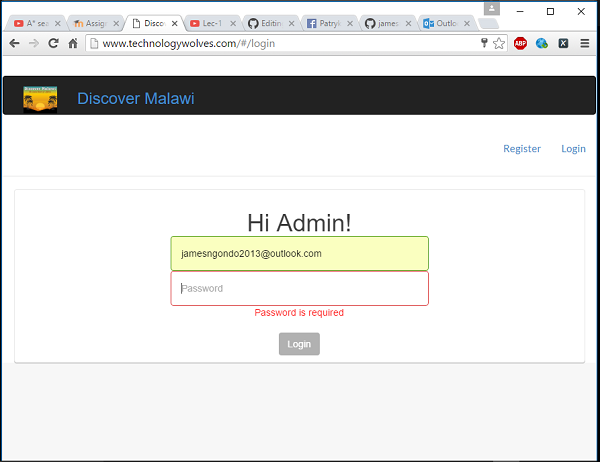
\includegraphics{img/login.png}
\end{center}
\begin{center}
	Figure 9: Admin Web App - Login Page
\end{center}
\paragraph{}

\subsubsection{New User Registration Page}
A successful login directs the admin user to the success page. While here, the admin can click on “Register New User” button to register a new user (admin). This will redirect the admin to a registration form page. All input fields in this form are validated using AngularJS form validation. The new user information is then sent to firebase database as shown in the figure below.

\begin{center}    
	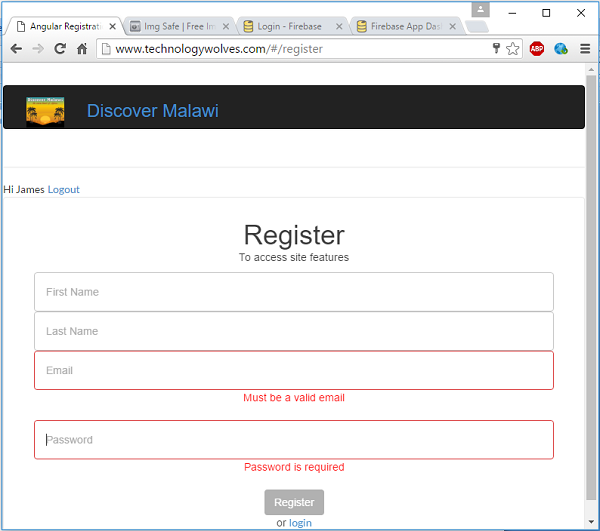
\includegraphics{img/register.png}
\end{center}
\begin{center}
	Figure 10: Admin Web App - Registration Page
\end{center}
\paragraph{}

\subsubsection{Success Page}
A successful login redirects the user to the success page. This is where the admin can view all data that the web application consumes from the firebase database. From here, the admin is able to navigate to other pages. After having access to data, the admin can now create, read, update and delete data from the database.

\begin{center}    
	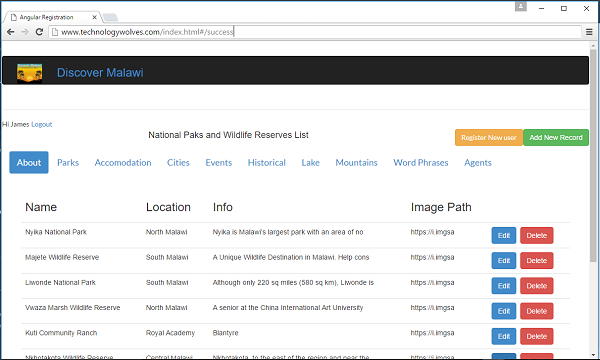
\includegraphics{img/success.png}
\end{center}
\begin{center}
	Figure 11: Admin Web App - Success Page
\end{center}
\paragraph{}

\subsection{Online Image Storage Server }
Img Safe is a free online image server that I used to host all the images for the application \cite{ImgSafe}.  One has to register an account first – using a valid email and password. Thereafter, you login using your details and upload your images. Firebase only stores data in a JSON format and therefore, raw images cannot be stored in it. Img Safe helps us get the image path in form of a URL and parse it to firebase as a value of an object. Every time we want to display images, firebase uses the image url to get to Img Safe server and retrieve the images that need to be displayed. Deleting image from the database will not affect images in Img Safe, but deleting images from Img Safe affects the entire app. See figure below.

\begin{center}    
	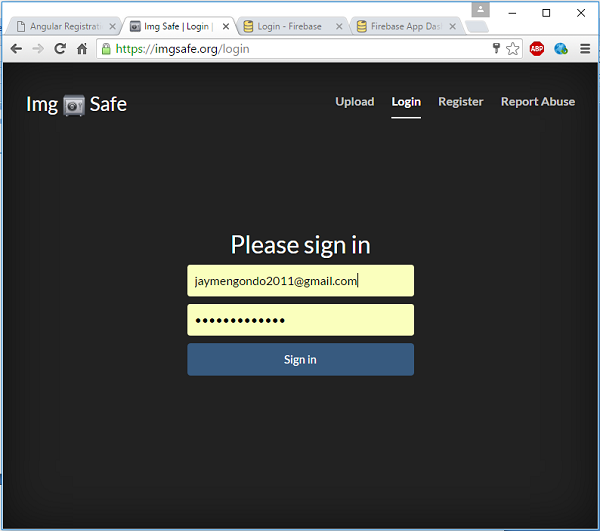
\includegraphics{img/imgsafe2.png}
\end{center}
\begin{center}
	Figure 12: ImageSafe Server - Login
\end{center}
\paragraph{}

Once logged in, the user can view all the images in their account and upload new images. Clicking on the image, will open that particular image in a seperate window where you can now get the URL (image path) for that image. The copied URL is then stored in the firebase database as value for a specific item.

\begin{center}    
	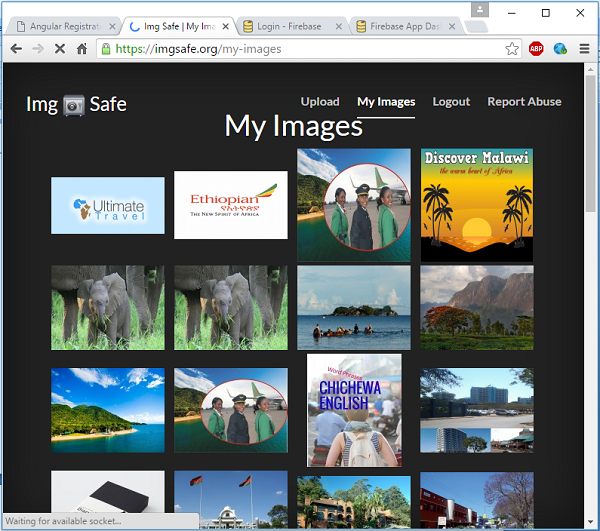
\includegraphics{img/imgsafe.png}
\end{center}
\begin{center}
	Figure 12: ImageSafe Server - My Account
\end{center}
\paragraph{}

\section{Front-end (Ionic App)}
The front-end is everything involved with what the user sees, including design. This is a graphical user interface designed and developed using AngularJS and Ionic framework. The front-end UI framework handles all of the look and feel and UI interactions the app needs in order to be compelling.
The mobile app uses the front end to pull data from firebase, as shown in the diagram below.

\begin{center}    
	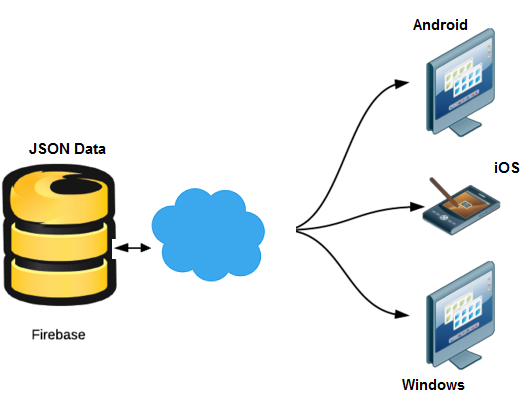
\includegraphics{img/frontend.png}
\end{center}
\begin{center}
	Figure 13: Ionic frontend architecture 
\end{center}
\paragraph{}
The front-end offers various functionalities to users giving them a feel of a personal native mobile application. This happens due to application’s graphical user interface design as it is optimized for displaying the content delivered in mobile devices. The application offers to users the option to define which information will be retrieved according to their preferences, and this information will be retrieved at the beginning of application use
The users can choose one of the following categories of places of interest: Lake Malawi, monuments, mountains, cities, hotels, weather, dictionary, Google Maps and travel agents. At each of those categories the user can choose the place of interest. Users can also create their own diary of events. The screenshots below describes how the app (front-end) looks like from the user perspective.

\subsection{Landing Page}
This page displays a list that contains all the places of interest and in Malawi and also allows the user to create their own diary of events. This page also has tabs at the bottom.

\subsubsection{Home Tab}
User taps on the home tab/ button at the bottom of the screen and they are redirected to the home page/ start page.

\begin{center}    
	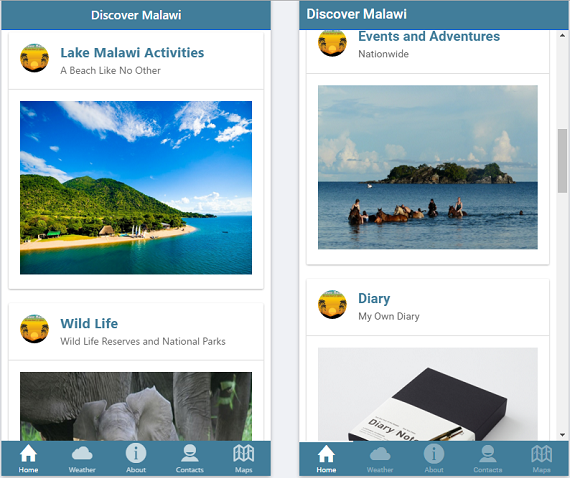
\includegraphics{img/startpage.png}
\end{center}
\begin{center}
	Figure 14: Home tab 
\end{center}
\paragraph{}

\subsubsection{Weather Tab}
The tab displays current weather forecast for four major tourist attraction cities in Malawi to help tourist plan their journey properly. 

\begin{center}    
	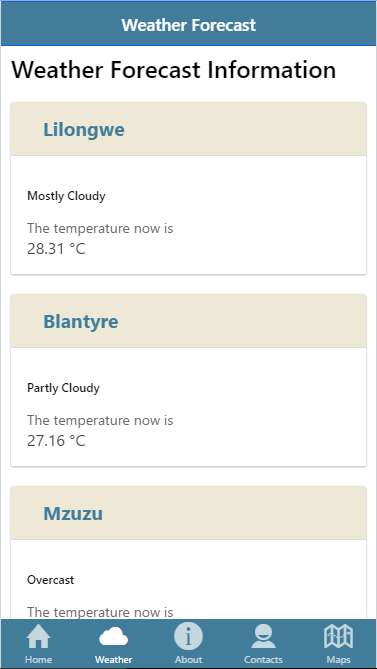
\includegraphics{img/weather.png}
\end{center}
\begin{center}
	Figure 15: Weather tab 
\end{center}
\paragraph{}

\subsubsection{About Tab}
The page displays information about Malawi such as language, culture, geography etc.

\begin{center}    
	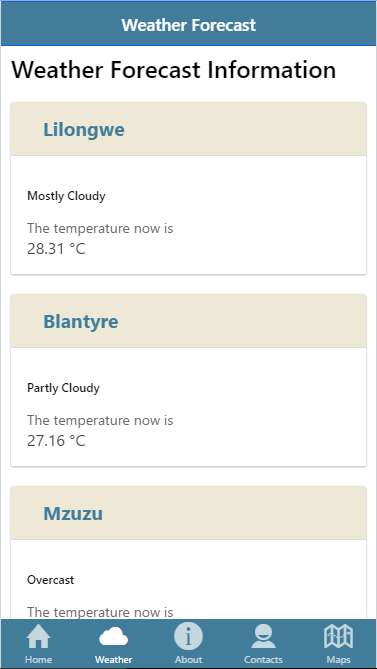
\includegraphics{img/weather.png}
\end{center}
\begin{center}
	Figure 16: About tab 
\end{center}
\paragraph{}

\subsubsection{Hotel / Accommodation Contacts}
This page displays the list of all hotels and accommodation places in Malawi. Each list item displays detailed information (name, location, website, email and telephone) about that particular hotel/ accommodation. The list has a functionality that allows user to mark some or all of the list items as favourites - indicated by a red star. When the user taps on the telephone item and the app is configured to auto dial the agent’s number. Upon tapping on the website, the instantly opens a web browser related to a particular hotel/ accommodation. 

\begin{center}    
	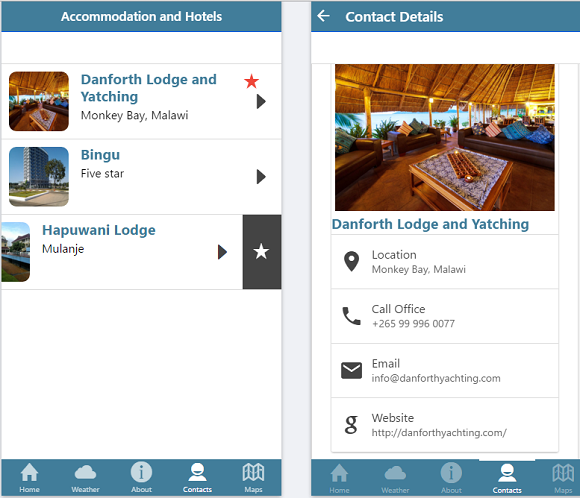
\includegraphics{img/contacts.png}
\end{center}
\begin{center}
	Figure 17: Contacts tab 
\end{center}
\paragraph{}

\subsubsection{Maps Tab}
The page displays the locations of Nation Parks and Wildlife Reserve in Malawi. The map has markers that display information related to a particular national park or wildlife reserve.

\begin{center}    
	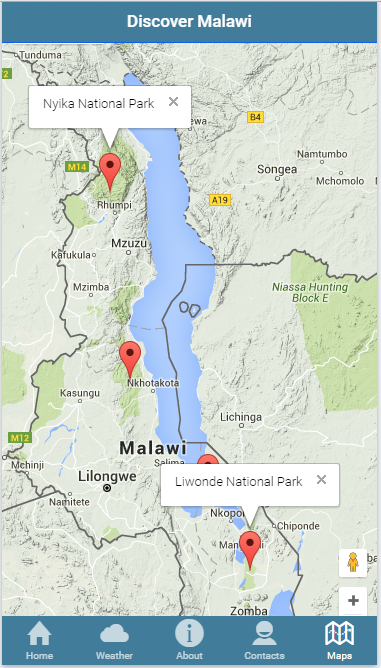
\includegraphics{img/maps.png}
\end{center}
\begin{center}
	Figure 17: Maps tab 
\end{center}
\paragraph{}

\subsection{Lake Malawi Activities}
This category displays all major events and activities that take along Lake Malawi. The list of activities is displayed on this page. The list has a functionality that allows user to mark some or all of the list items as favourites - indicated by a red star. The user taps on each list item and it displays detailed information for that particular item. The detailed info page allows the user to share information via twitter, facebook and other social sharing apps that are installed in the user’s device.

\begin{center}    
	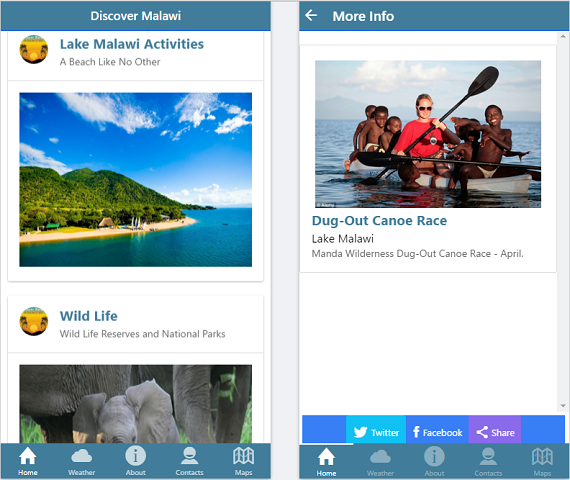
\includegraphics{img/lakemalawi_info.png}
	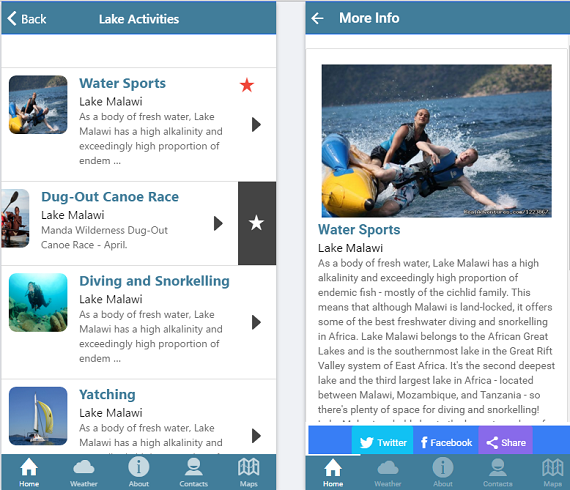
\includegraphics{img/lakemalawi.png}
\end{center}
\begin{center}
	Figure 18: Lake Malawi Activities 
\end{center}
\paragraph{}

\subsection{National Parks and Wildlife Reserves}
This category displays all games reserves and national parks in Malawi. The user can mark some or all of the list items as favourites indicated a red star. The user taps on each list item and it displays detailed information for that particular item. The detailed info page allows the user to share information via twitter, facebook and other social sharing apps that are installed in the user’s device.

\begin{center}    
	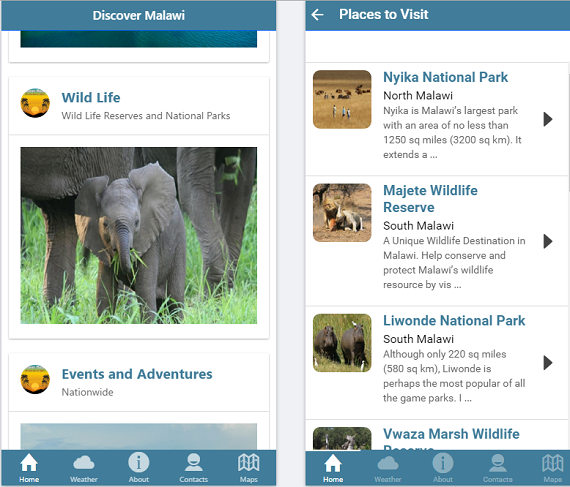
\includegraphics{img/wildlife1.png}
	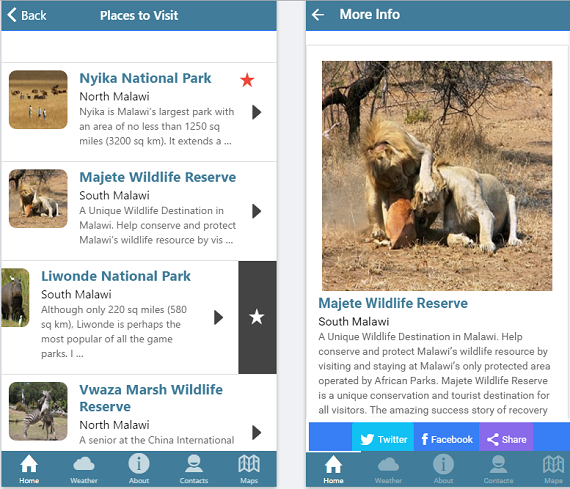
\includegraphics{img/wildlife.png}
\end{center}
\begin{center}
	Figure 19: National Parks and Wildlife Reserves 
\end{center}
\paragraph{}

\subsection{Events and Adventures}
This category displays all events and adventures that take place in Malawi at different seasons of the year. The list has a functionality that allows user to mark some or all of the list items as favourites - indicated by a red star. The user taps on each list item and it displays detailed information for that particular item. The detailed info page allows the user to share information via twitter, facebook and other social sharing apps that are installed in the user’s device.

\begin{center}    
	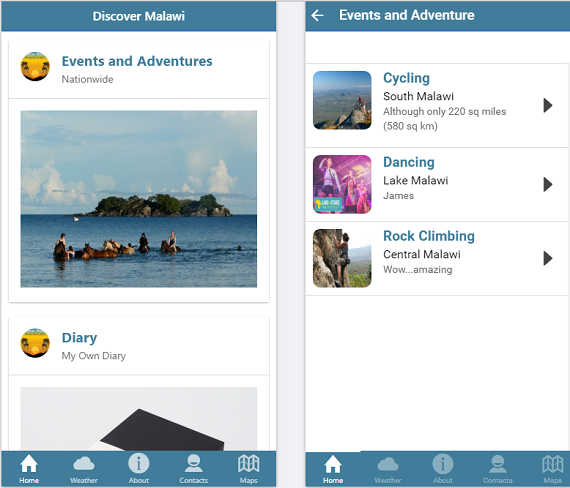
\includegraphics{img/events.png}
	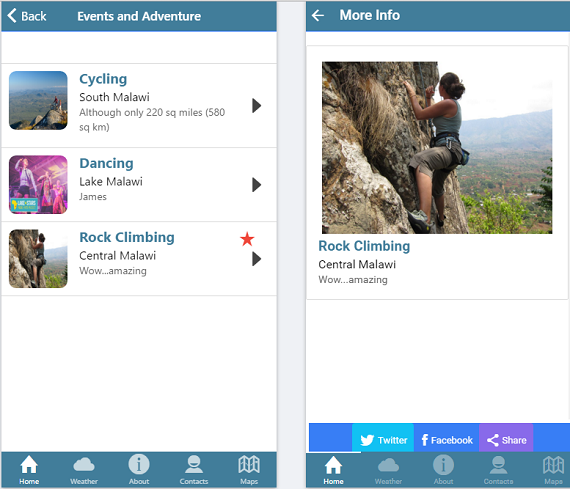
\includegraphics{img/events2.png}
\end{center}
\begin{center}
	Figure 20: Events and Adventures 
\end{center}
\paragraph{}

\subsection{Events Notes/ Diary}
Users can create their own diary of events in advance prior to arriving in Malawi of during the holiday stay. All the notes create d are stored locally in the user devices. The code snippet below is used to store data locally on the user device.

\begin{minted}{javascript}
app.factory('NoteStore', function($firebaseArray, $firebaseObject){
	//retrieve notes from local storage
	var notes = angular.fromJson(window.localStorage['notes'] ||'[]');
	// store notes in local storage
	function persist()
	{
		window.localStorage['notes'] = angular.toJson(notes);
	}   
});
\end{minted}
 
When the user clicks on an item, they are directed to “Edit Page” where they can edit/ update their notes. The user may delete, edit or re-order their notes at any time.

\begin{center}    
	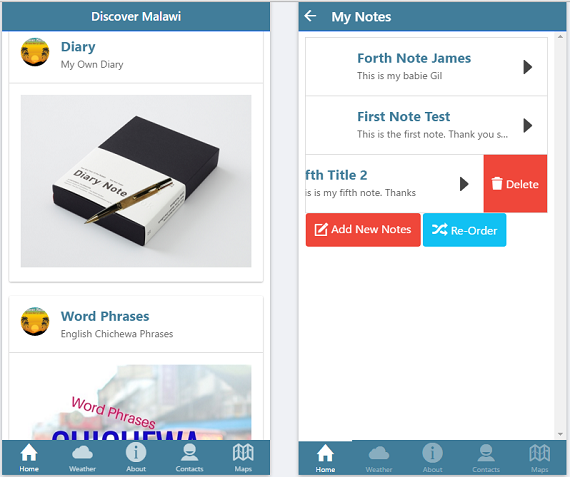
\includegraphics{img/diary.png}
	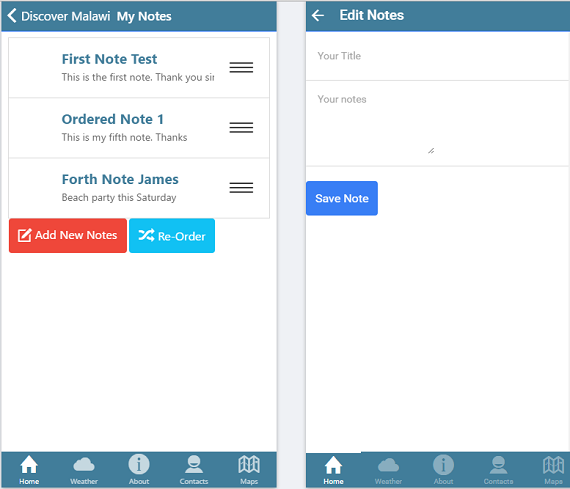
\includegraphics{img/diary3.png}
\end{center}
\begin{center}
	Figure 21: Event notes / diary 
\end{center}
\paragraph{}

\subsection{Dictionary/ Word Phrases}
The dictionary provides most of the commonly used English and Chichewa word phrases that are familiar with tourist. In this page provides a functionality that allows users to filter words/ phrases based on their search criteria. 

\begin{center}    
	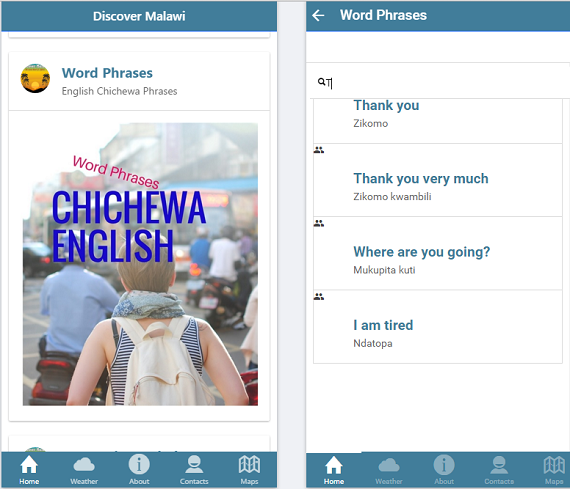
\includegraphics{img/dictionary.png}
\end{center}
\begin{center}
	Figure 22: Word Phrases - Dictionary 
\end{center}
\paragraph{}

\subsection{Mountains and Plateaus}
This category displays all mountains and plateaus in Malawi. The list has a functionality that allows user to mark some or all of the list items as favourites - indicated by a red star. The user taps on each list item and it displays detailed information for that particular item. The detailed info page allows the user to share information via twitter, facebook and other social sharing apps that are installed in the user’s device.

\begin{center}    
	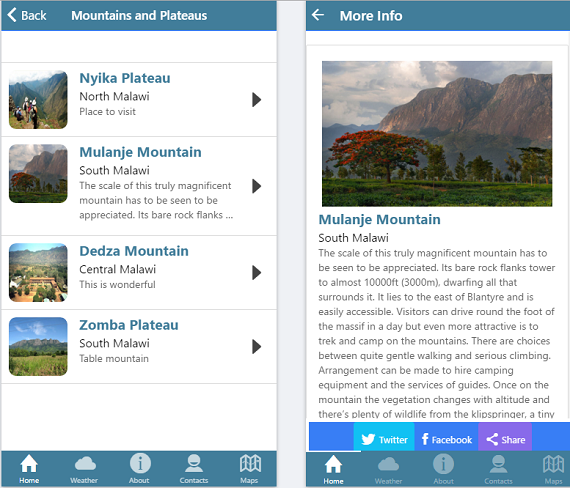
\includegraphics{img/mountains.png}
\end{center}
\begin{center}
	Figure 23: Mountains and Plateaus 
\end{center}
\paragraph{}

\subsection{Historical Sites and Monuments}
This category displays all Historical Sites and Monuments in Malawi. The list has a functionality that allows user to mark some or all of the list items as favourites - indicated by a red star. The user taps on each list item and it displays detailed information for that particular item. The detailed info page allows the user to share information via twitter, facebook and other social sharing apps that are installed in the user’s device.

\begin{center}    
	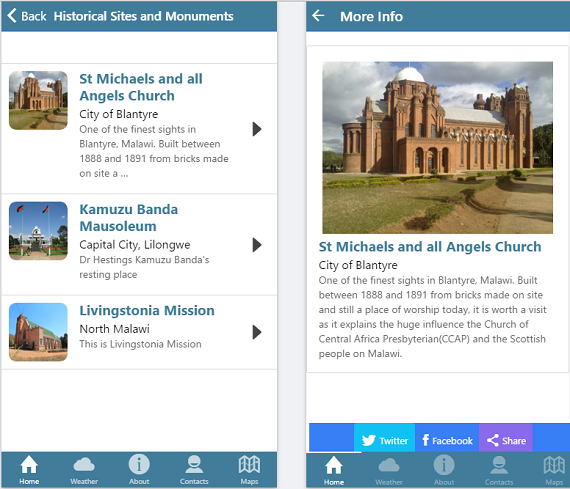
\includegraphics{img/history.png}
\end{center}
\begin{center}
	Figure 24: Historical Sites and Monuments 
\end{center}
\paragraph{}

\subsection{Cities}
This category displays major cities in Malawi. The list has a functionality that allows user to mark some or all of the list items as favourites - indicated by a red star. The user taps on each list item and it displays detailed information for that particular item. The detailed info page allows the user to share information via twitter, facebook and other social sharing apps that are installed in the user’s device.

\begin{center}    
	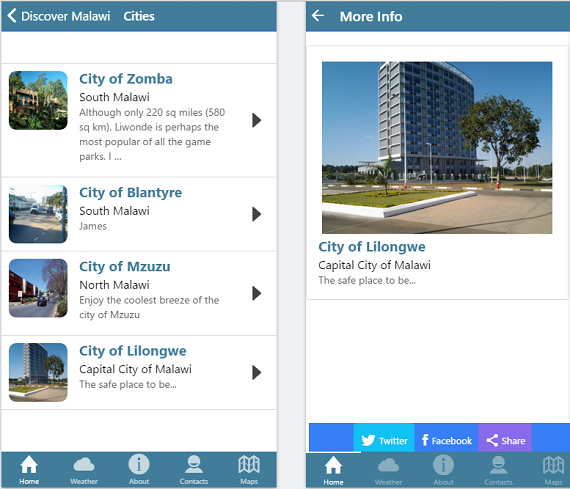
\includegraphics{img/cities.png}
\end{center}
\begin{center}
	Figure 25: Cities 
\end{center}
\paragraph{}

\subsection{Travel Agents}
This category displays most of the travel agents in Malawi. This will help tourists in case they want to make travel arrangements. Each list item displays detailed information (name, location, website, email and telephone) about travel agents. The list has a functionality that allows user to mark some or all of the list items as favourites - indicated by a red star. When the user taps on the telephone item and the app is configured to auto dial the number. Upon tapping on the website, the instantly opens a web browser related to a particular travel agent.

\begin{center}    
	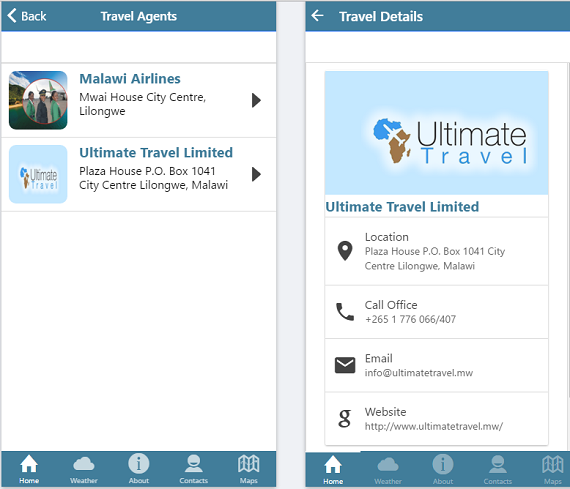
\includegraphics{img/travel.png}
\end{center}
\begin{center}
	Figure 26: Travel Agents 
\end{center}
\paragraph{}



\chapter{System Evaluation}
As many pages as needed.
This section evaluates how the system functions. The evaluation itself will focus on the following: 
\begin{itemize}
	\item Robustness.  
	\item Performance based on space and time.
	\item Outcomes / outputs of the system.
\end{itemize}

I will also hight any limitations or opportunities based on the technologies used.

\paragraph{}
\section{Robustness}
The system has proven to be robust in the sense that it does not break down easily and is not wholly affected by a single application failure. As mention earlier in this report that the system comprises different components put together and constantly communicating with each other, i.e. the system backend and the frontend. The backend itself has proven to be more reliable simply because its running on firebase, which happens to be the most reliable Backend as  Service (BaaS). It is unlikely that firebase can easily break down and affect the entire system. Firebase was designed for continuous operation with a very low failure rate and features such as automatic backup of file systems. The Admin web app \cite{hosting24} which lets the admin interact with the database has also proven to be robust in the sense that it was designed to run on almost every web browser (Chrome, Firefox, Internet Explorer and Safari) without causing any problems. 
The code snippet below is a Selenium Web driver test written in Java to test the web app in firefox web browser. This code snippet will take in an email address and password, opens the browser and login itself successfully.
\begin{minted}{javascript}
public static void discoverMalawiSignIn() {
	FirefoxDriver driver = new FirefoxDriver();
	driver.get("http://www.technologywolves.com/#/login");
	WebElement username = driver.findElement(By.name("email"));
	username.sendKeys("jamesngondo2013@outlook.com");
	WebElement button = driver.findElement(By.name("password"));
	button.click();
	
	WebElement password = (new WebDriverWait(driver, 30))
	.until(ExpectedConditions.presenceOfElementLocated(By.name("password")));
	password.sendKeys("g00304277");
	
	WebElement btnLogin = driver.findElementByClassName("btn");
	btnLogin.click();
	
	driver.manage().window().maximize();
	
	sleep();
	
	// click each tab
	WebElement btn;
	WebDriverWait wdw = new WebDriverWait(driver, 30);
	
	WebElement navBar = wdw.until(ExpectedConditions.presenceOfElementLocated(By.className("nav")));
	String[] allLinks = navBar.getText().split("\n");
	for (int i = 0; i < allLinks.length; i++) {
		System.out.println(i + ": " + allLinks[i]);
		driver.findElement(By.linkText(allLinks[i])).click();
		sleep();
	}
	
	sleep();
	
	WebElement myDynamicElement = (new WebDriverWait(driver,
	30)).until(ExpectedConditions.presenceOfElementLocated(By.linkText("Logout")));
	driver.findElement(By.linkText("Logout")).click();
	
	
}
	
public static void sleep()
{
	try {
		Thread.sleep(1000);
	} catch (InterruptedException e) {
		e.printStackTrace();
	}
}
\end{minted}

The web app may also function on its own - its break down or malfunctioning may not affect the database or frontend (ionic app). The ionic app (frontend) is also designed to run on major mobile platforms such Android and iOS. Black-box testing was used while working on the ionic app. This method of software testing was focused on examining the functionality of an application (ionic app) without peering into its internal structures. In this regard, the ionic application project compiled to android platform and an .apk file was created and installed in several android devices where users were able to interact with the app. We discovered that the app was user friendly and responsive in all of the devices that were used for testing. The project was also deployed using ionic cordova framework emulator for both Android and iOS platforms that allows the developers to see how the app may look like or function on certain platforms. The result was successful. 

\section{Performance based on space and time}
\paragraph{Space}
- In terms of space complexity, this system has been designed in such a way that it does not use up much memory space. The database itself is stored as a JSON file that is approximately 38 KB in size and this holds all the data that is consumed by the frontend. More and more data can be added to the database without affecting memory space in the database. The database is more efficient even when more data is added to it. 
The admin web application that lets the administrators interact with the database is also designed not to take much space. With the size of approximately 958 KB, its easier for the website to be deployed to any web server or hosting site without having to worry about space. 
The size of the .apk file is small enough to be installed in any device without having to worry about its size and space to be used.

\paragraph{Time}
- In terms of time complexity, the system does not take time at all to load up. Tha mobile app (ionic) itself takes performs very well when retrieving data from firebase database. When firebase is accessed through a client library, changes to data are synchronized in real-time to clients within milliseconds. Depending on network’s speed, propagating changes from one device to others can take around 100ms or less.
Admin login from the web application is also pretty fast. Data retrieval is very fast. Overall performance of the application in terms of time and and space complexity is very efficient.

\section{Outcomes / outputs of the system}
The overall output of the system is very satisfactory when measured against the main objectives of the system. Most of the functionalities of the system perform as intended. 

\section{Limitations and opportunities}
\paragraph{Limitations} 
The system runs on firebase as a backend service and therefore, you can have only 50 active users at once and only 5GB data can be transferred within one month. You can store only 100 MB of data on a free plan. The major disadvantage to Firebase is that it isn't free, and if you have significant traffic it can quickly become fairly expensive. 
Also, firebase is a third party server-side application that provides basic database queries. Very complex queries can not be achieved with firebase. In case firebase goes down, the application will not function properly since it relies on the data from firebase.
Firebase does not offer offline support for android ionic apps (angularjs) at the moment even though they have offline SDKs for android platforms developed in Java. In this case I have decided to store all data into the device's local storage where it can be fetched when the app is offline. 
The application also relies on imgsafe - an online image server that stores all the images used by our application. Failure of this server may also affect the entire frontend since all images for the app are stored online.

\paragraph{Opportunities}
- The system uses Firebase that provides client-side libraries for Android, iOS, all major JavaScript browser frameworks, Node.js, and Java. These libraries give clients impressive real-time data-synchronization capabilities. The Firebase platform is essentially a fully-hosted service that stores JSON in a tree accessed via RESTful URLs. One thing to note is that when you load a node in the tree, you get all of the data under that node. 
The mobile application is developed using ionic framework - a cross platform and lets you write the same app once for multiple platforms. Ionic not only comes with well documented markup and CSS, but also JavaScript design patterns to help you build some serious apps with similar concepts to iOS and Android.
Firebase provides a full set of tools for managing the security of your app. These tools make it easy to authenticate our users, enforce user permissions, and validate inputs. Hence you will save time building your own backend service.


\chapter{Conclusion}
This application will provide a better user experience by taking advantage of newest technologies in order to promote Lake Malawi, mountains, wildlife reserves, cities, hotels, museums and the cultural heritage.
The mobile application has been developed using ionic framework. This is a cross platform framework that has helped me develop the same app once for multiple platforms. The advantage is that Ionic not only comes with well documented markup and CSS, but also JavaScript design patterns to help you build some serious apps with similar concepts to iOS and Android.
Data being consume by this application is retrieved from the backend service (Database) the first time the user uses the application.
The database itself is running on Firebase, a real-time cloud data service and provides an API that stores and syncs data across multiple clients or devices and it serves millions of users in no time. Firebase database is stored as JSON and synchronized in realtime to every connected client. The data in the database can be easily exported into a JSON file that can be imported into MongoDB without any problems.

The system has been designed in such a way that it does not use up much memory space. The database itself is stored as a JSON file, approximately 38 KB in size and this holds all the data that is consumed by the frontend. More and more data can be added to the database without affecting memory space in the database. The database is more efficient even when more data is added to it. 
The administrator web application also designed not to take much space. With the size of approximately 958 KB, its easier for the website to be deployed to any web server or hosting site without having to worry about space. 
The size of the discovermalawi.apk file is small enough to be installed in any device without having to worry about its size and space to be used.
The system limitations comes as a result of firebase only allowing a limited number of users and also the amount of data that can be transfered within a month in case of free price plan users.This simply means that as a free user, you may be limited in some ways when it comes to usage. 

\chapter{Recommendations}
At a later stage during the development process, I discovered that firebase does not offer offline support for angular ionic apps (angularjs) at the moment even though they have offline SDKs for android platforms developed in Java. I figured out that the other way to go about this is to save data in local storage after reading from firebase. In this case I have decided to store all data into the device's local storage where it can be fetched when the app is offline. The only tricky part of this exercise is that I have to map each individual image to a specific data that corresponds with it. This development is under way and it will be completed in no time.

\chapter{Appendix}
\paragraph{Project Source Code Link:}
https://github.com/jamesngondo2013/DiscoverMalawi

\paragraph{Project Documentation Link:}
 https://github.com/jamesngondo2013/Discover-Malawi-Project-Documentation
 
 \paragraph{Admin Panel Web App Link:}
 http://www.technologywolves.com/
